\documentclass[11pt,a4paper]{report}
\usepackage[latin1]{inputenc}
\usepackage{hyperref}
\hypersetup{
    colorlinks,
    citecolor=black,
    filecolor=black,
    linkcolor=black,
    urlcolor=black
}
\usepackage{amsmath}
\usepackage{amsfonts}
\usepackage{amssymb}
\usepackage{acronym}
\usepackage{graphicx}
\author{Diogo Curto}
\title{Low-Power Systems Evaluation}
\date{Original date: September 09, 2014 \\ Last Modified: December 02, 2014}

\begin{document}

\begin{titlepage}
\hypersetup{pageanchor=false}
\maketitle
\hypersetup{pageanchor=true}
\end{titlepage}

\tableofcontents

\chapter{Low-power systems and applications}

When defining a system as being low-power it comes down to the application. Every one has a definition for what it needs to be low-power. In most cases, a low-power application is defined by its efficiency. 
The system needs to get the most work done in the less time as possible, with the minimum use of CPU while working as slow as possible and consume only the strictly necessary power \cite{Wong2009}.


With this thoughts in mind, is clear that low-power systems require optimization at all levels, from the microcontroller architecture up through the application layer.

Throughout this chapter will be introduced the main power categories and design techniques for microcontroller based systems and applications to be as efficient as possible.

\section{Power Categories}\label{Power_Categories}
There are two real factors involved in the application design: dynamic power consumption when it is running and static power for when it is asleep \cite{SedraSmith}.

\begin{equation} \label{Pdynamic}
P_{dyn} =\alpha \times f \times C \times V^2
\end{equation}

Dynamic power, as expressed in equation~\ref{Pdynamic}, is affected mainly by the supply voltage and the charging and discharging of capacitances at the clock frequency.
The parameter $\alpha $ is a scaling factor that varies when considering an entire MCU. This is the power consumed when the CPU is running and processing data. From a systems designer point of view, the changeable parameters, not arbitrarily because they are dependent on each other, during system design are the supply voltage and operating frequency. 

In a more global view, dynamic power is not only associated to the CPU itself, but also to the peripherals, both internal and external. 
This is important since most microcontrollers have the ability to shutdown internal peripherals completely in order to save power. 

External peripherals can also be shutdown by using, for instance, I/O pins to power those devices, or even to control a transistor working as switch.

Static power encompasses the power required to maintain proper system operation while code is not actively running and is highly dependable on voltage, temperature, leakage and bias currents for analog circuits. This is considered when the CPU is in standby (idle) and normally waiting for an event to occur. In battery applications this is the state in which the CPU stays longer and therefore consumes the most significant battery power. Most applications need memory to work properly and therefore data retention power must be taken into account when discussing static power.
 
In terms of embedded systems, the most common practice is to discuss current consumption of each part instead of power consumption due to the fact that normally, the voltage supply is fixed to a predetermined range and the most changing variable is current. Therefore, over this text, device characterization will be expressed in current consumption. 

\section{Design Techniques}

When designing a low-power system, the first step is normally to do a power budget. Is necessary to evaluate
the needed or allowable power modes and estimate for how long the system will be running to accomplish the determined objectives. It is also important to consider the use of the peripherals: the time they will run in each different power mode and so on \cite{Ivey2011}.

\begin{figure}[ht!]
\centering
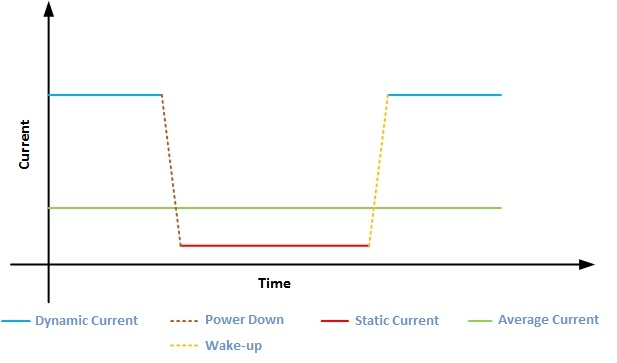
\includegraphics[width=0.9\linewidth]{Current_over_time.jpg}
\caption{Generic system current consumption }
\label{fig:Current_over_time}
\end{figure}

\begin{equation} \label{avg_current}
I_{AVG} = \dfrac{I_{dyn}\times t_{dyn} + I_{st}\times t_{st}}{t_{dyn} + t_{st}}
\end{equation}

After this, it is necessary to calculate the current consumption of each mode and the time spent on each mode to get an overall estimation of  average current consumption for the application as shown in figure~\ref{fig:Current_over_time} and calculated in equation~\ref{avg_current}.

This allows us to get an overall view in what is needed from the power-supply and the expected battery life. It also allows to get a good view of what parts of the system need more focus in order to minimize current consumption.

With these thoughts in mind, over the next sections, will be presented microcontroller features capable of managing the current consumption of specific modules and tasks.

\subsection{Supply Voltage Range}\label{Supply_voltage_range}

When considering a reduction in the supply voltage in order to reduce the current consumption, there is a limitation to it that cannot be overlooked. The minimum supply voltage is limited by the operating frequency, that is, to reduce the supply voltage is also necessary to change the frequency. As an example in figure \ref{fig:frequency_over_voltage} is shown the frequency limitations depending on the supply voltage.

\begin{figure}[ht!]
\centering
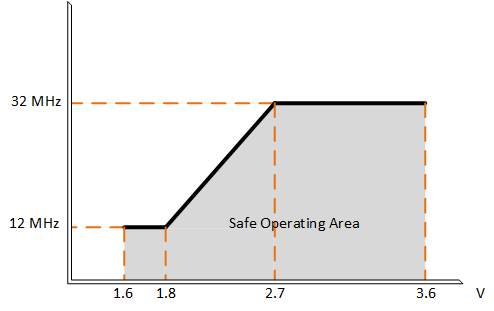
\includegraphics[width=0.9\linewidth]{./frequency_over_voltage}
\caption{Frequency vs Supply voltage. Figure 32-22 \cite{Atmel_ATxmegaxxx}}
\label{fig:frequency_over_voltage}
\end{figure}

\subsection{Clock Speed}

As discussed in the section~\ref{Power_Categories}, the clock speed is an important factor to reduce current consumption. When considering an application that runs for a specific time and then goes back to sleep, is important to consider the trade-off between speed and current consumption, that is, evaluate what consumes more current: execute at really low speeds or run fast and then go to sleep for a longer period. 

In order to explain the statement above, an example is provided in figure \ref{fig:Average_power_vs_work_load_31K} for active current consumption. This figure was obtained by taking a generic application with a certain amount of work that needs to run every ten seconds for five different clock speeds:
 
\begin{eqnarray}\nonumber
\left\{\begin{matrix}
32 \text{ MHz} &-& \text{IAVG32}	\\ 
8 \text{ MHz} &-& \text{IAVG8}	\\ 
2 \text{ MHz} &-& \text{IAVG2}	\\ 
1 \text{ MHz} &-& \text{IAVG1}	\\ 
31 \text{ kHz} &-& \text{IAVG31k}
\end{matrix}\right.
\end{eqnarray}

As can be seen, executing at 31 KHz is always worst than higher speeds. This occurs due to the very low execution speed, since the microcontroller is always working instead of in a Deep-Sleep state. 

\begin{figure}[ht!]
\centering
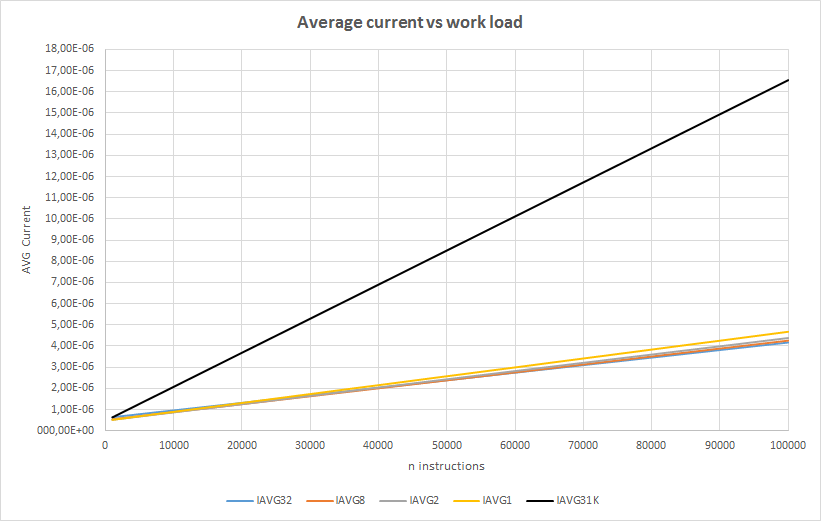
\includegraphics[width=0.9\linewidth]{./Average_power_vs_work_load_31K}
\caption{Clock speed average active current vs work load. CH 32 \cite{PIC24FJ128GA204} \cite{Power_saving_deep_sleep}}
\label{fig:Average_power_vs_work_load_31K}
\end{figure}

A better overview of this case is shown in figure \ref{fig:Average_power_vs_work_load}. Here, the 31 KHz average current was removed. As the work load starts to increase, the most efficient frequencies are the highest. This indicates that executing at low speeds is only better if the work load is small. 

\begin{figure}[ht!]
\centering
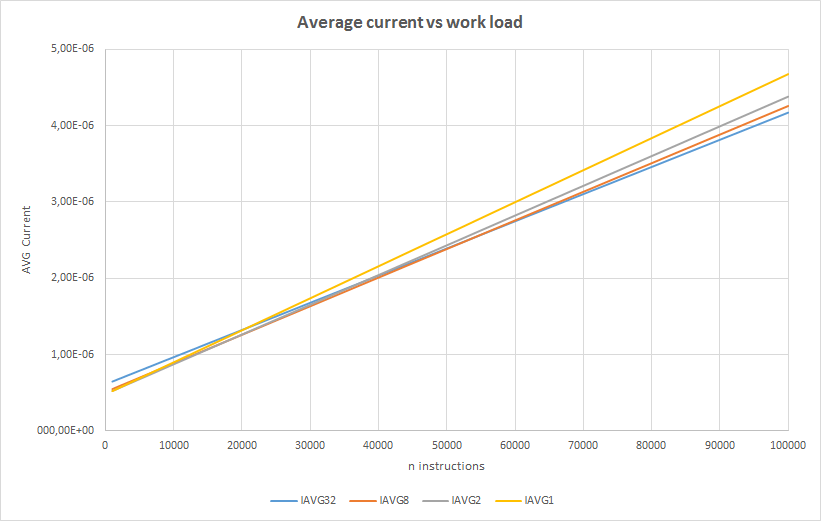
\includegraphics[width=0.9\linewidth]{./Average_power_vs_work_load}
\caption{Clock speed average active current vs work load. CH 32 \cite{PIC24FJ128GA204} \cite{Power_saving_deep_sleep}}
\label{fig:Average_power_vs_work_load}
\end{figure}

These figures were obtained based on equation \ref{avg_current}. More explicitly:

\begin{eqnarray}\nonumber
\left\{\begin{matrix}
i_{dyn}(f) &=& i_{DD}(f) \\
t_{dyn}(f) &=& t_{\text{WU}} + t_{\text{n inst}}(f) + t_{\text{PD}}(f)\\
I_{st} &=& I_{\text{DS}} \\
t_{st}  &=& t_{\text{DS}} \\
t_{dyn}(f) + t_{st} &=& 10 \text{ s} 	
\end{matrix}\right.
\end{eqnarray}

Another important aspect of frequency reduction to consider is the fact that in order to maintain the logic level, a certain amount of current must be used. This is necessary to maintain the charge level of the intrinsic capacitances of the microcontroller (recall equation \ref{Pdynamic}). For lower frequencies, this logic level must be held for more time, increasing the current consumption. When using higher frequencies, the voltage (logic) level decay is negligible making these more efficient than lower frequencies. An example is shown in figure \ref{fig:system_efficiency_silicon_labs}.

When considering running the application at higher speeds there is another factor that rises as shown in section \ref{Supply_voltage_range}: Most microcontrollers need higher supply voltages in order to run faster. Therefore, to avoid errors in code execution, another feature must be used: A low-voltage detector, that enables, for instance, to reduce clock speed in runtime and therefore extend battery life.
There is another feature useful both at higher and lower speeds called the Brown-out Reset. This allows to protect the application from errors as batteries die, or when high peaks of dynamic current bring the supply voltage to an unsupported level, resetting the microcontroller in both cases.

In some applications, the relevant mode is not when the application is running (active mode). This happens when the system spends a large portion of his time in a Sleep/Low-Power mode making this the most relevant mode for current consumption. Meaning that the most important mode to consider really depends on the duty cycle between the various sleep and active modes.
  
\begin{figure}[ht!]
\centering
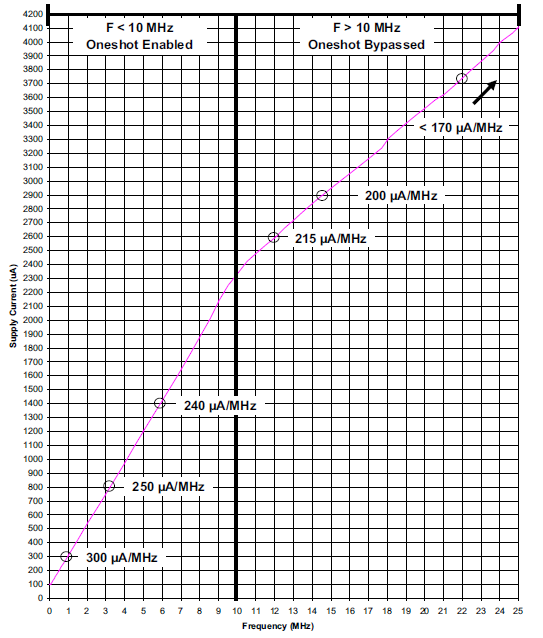
\includegraphics[width=0.9\linewidth]{./system_efficiency_silicon_labs}
\caption{Active Mode Current Efficiency. Figure 4.1 \cite{C8051F93x}}
\label{fig:system_efficiency_silicon_labs}
\end{figure}


\subsection{Wake-up time}


Wake-up time refers to the transition from low-power to active modes. For systems with short active windows the wake-up process consumes a similar amount of current as normal operation. 
The more functions that are turned off, the less current the chip will consume, but the longer it will take it to wake up.

Another important factor is the oscillator start-up delay, which depends on the clock source as well as other frequency dividers/multipliers in the path.
Wake-up time will usually be the limiting factor that determines which low-current mode can be used at a given time in the application. 
In order to minimize this issue, some additional peripherals can be used. For instance, an internal voltage regulator that allows to maintain the internal capacitances charged, reducing wake-up time in 200 $\mu s$. 

\begin{figure}[th!]
\centering
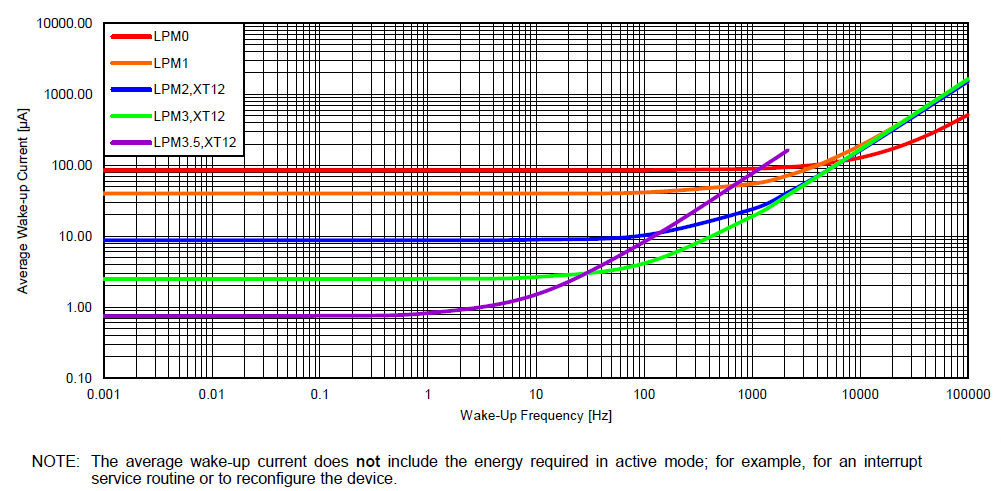
\includegraphics[width=0.9\linewidth]{Average_LPM_Currents}
\caption{Average LPM Currents vs Wake-up Frequency at 25 �C . Figure 5-3 \cite{MSP430698} } 
\label{fig:Average_LPM_Currents}
\end{figure}

This figure comes in the sequence of figures \ref{fig:Average_power_vs_work_load_31K} and \ref{fig:Average_power_vs_work_load}. EXPLICAR!!!!!!!

\subsection{Instruction Set Architecture}


When evaluating current consumption of a microcontroller, one of the key aspects to take into account is the instruction set. That is, the amount of actual work done per unit of energy consumed. The clocking scheme - ratio between the input system clock and the instruction clock frequencies, cycles per instruction and available instructions have major impact on current consumption.

For instance the ALU (Arithmetic Logic Unit), is one of the most important components of a CPU. The level of complexity has a major impact on current consumption. When an ALU is highly complex with very built-in capabilities, for instance, multiplier/divider units, floating point and registry calculation, and so on, this not always is good in therms of current consumption. 
If the application requires very little of these features, a good portion of current is wasted. 
But if the application requires all these features, and they are unsupported by the ALU, they must be decomposed into simpler instructions, which may require a large number of clock cycles to process. 

This means that the microcontroller must be adjusted for the application in order to maximize current efficiency.

In order to materialize the above statements, for instance, in some devices, Texas Instruments \cite{MSP430698}, opted to reduce CPU (ALU) complexity and incorporated an Hardware Multiplier (1 CPU Cycle\footnote{Using Direct Memory Access}) as a peripheral with no direct support for division. On the contrary, Microchip Technology \cite{PIC24FJ128GA204}, added hardware support for both multiplication (1 CPU cycle) and division (18 CPU cycles). 

With no direct comparison intended beyond the point of giving two examples, these architectural choices clearly show that these two different devices are useful in different applications.

 

\subsection{Data Retention}

Most microcontrollers provide two main types of sleep modes. The first is a light-sleep mode, in which the MCU core is stopped, peripherals are disabled, and clock sources are turned off. However, the MCU stays powered up, preserving the contents of registers and SRAM making the wake-up process faster.

The second, is a deep-sleep mode, in which the entire MCU is powered down and SRAM contents are lost. In order to avoid the loss of data, is necessary to save the needed data to Flash or EEPROM memories. When the CPU wakes-up the data needs to be restored in order to resume operation. Unfortunately, due to high write/erase time and current spent on this process, the energy used is substantial. 

\subsubsection{SRAM, EEPROM, Flash and FRAM}


Although SRAM is the type of memory most used in microcontrollers, Ferroelectric RAM is the most adequate for low-power applications as shown in table \ref{memoriescomparison}.

\begin{table}[ht!] \caption{Comparison between different types of memories. \cite{FRAMFujitsu} \cite{FRAMPres}}
\begin{tabular}{|l|c|c|c|c|}
\hline
                  & SRAM      & EEPROM               & FRAM                  & FLASH                \\ \hline
Type              & Volatile  & Non-Volatile         & Non-Volatile          & Non-Volatile         \\ \hline
Write Cycle       & 55 ns     & 5 ms                 & 150 ns                & 10 $\mu$s                \\ \hline
R/W Cycles & Unlimited & $10^6$ & $10^{13}$ & $10^5$ \\ \hline
Read Current      & 40 mA     & 5 mA                 & 4 mA                  & 12 mA                \\ \hline
\end{tabular}\label{memoriescomparison}
\end{table}


\bibliography{TESE}
\bibliographystyle{ieeetran}

\end{document}

